\documentclass[tikz,border=10pt]{standalone}
\usepackage{amsmath}
\usetikzlibrary{angles}
\begin{document}
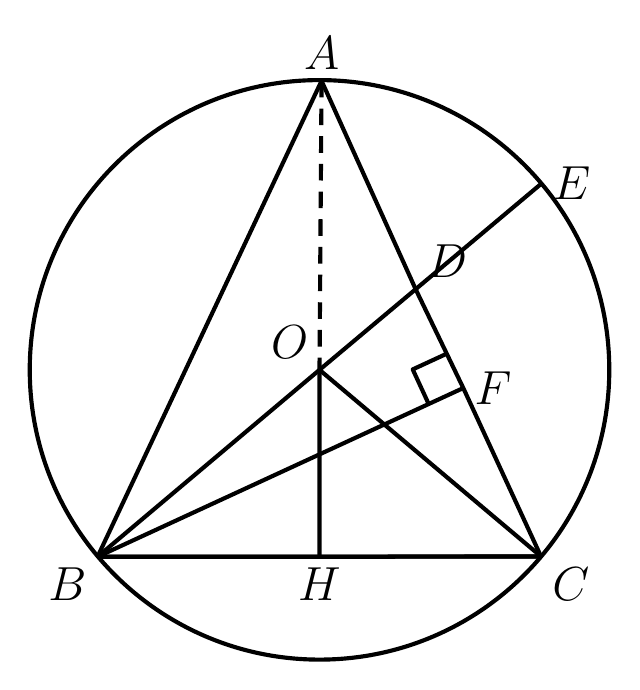
\begin{tikzpicture}[line width=1.5pt, line join=round]
\coordinate (A) at (0.007,3.332);
\coordinate (B) at (-2.838,-2.712);
\coordinate (C) at (2.794,-2.708);
\coordinate (D) at (1.202,0.686);
\coordinate (E) at (2.801,2.029);
\coordinate (F) at (1.807,-0.569);
\coordinate (H) at (-0.020,-2.712);
\coordinate (O) at (-0.019,-0.338);




\draw (O) circle (3.680);


\draw (A) -- (B);
\draw (B) -- (C);
\draw (A) -- (D) -- (F) -- (C);   


\draw (B) -- (F);
\draw (B) -- (O) -- (D) -- (E);   


\draw (B) -- (H) -- (C);
\draw (H) -- (O);
\draw (C) -- (O);


\draw[dash pattern=on 6pt off 4pt] (A) -- (O);


\draw pic[draw, angle radius=0.484cm] {right angle=A--F--B};


\node[above] at (A) {\fontsize{16.5}{19.8}\selectfont $A$};
\node[below left] at (B) {\fontsize{16.5}{19.8}\selectfont $B$};
\node[below right] at (C) {\fontsize{16.5}{19.8}\selectfont $C$};
\node[above right] at (D) {\fontsize{16.5}{19.8}\selectfont $D$};
\node[right] at (E) {\fontsize{16.5}{19.8}\selectfont $E$};
\node[right] at (F) {\fontsize{16.5}{19.8}\selectfont $F$};
\node[below] at (H) {\fontsize{16.5}{19.8}\selectfont $H$};
\node[above left] at (O) {\fontsize{16.5}{19.8}\selectfont $O$};
\end{tikzpicture}
\end{document}